\documentclass[tikz]{standalone}
\usepackage{amssymb}
\usepackage{tikz}
\usetikzlibrary{3d}

\begin{document}

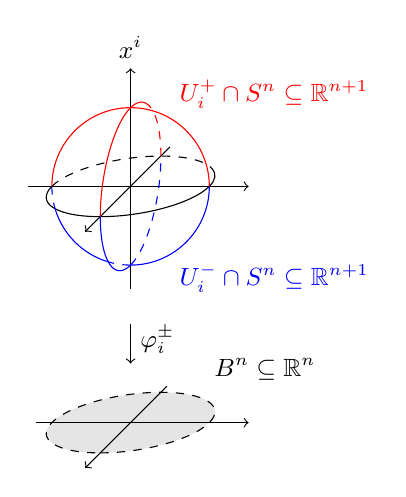
\begin{tikzpicture}[every node/.style={font=\small}]

  \draw[->] (-1.3,0,0) -- (1.5,0,0);
  \draw[->] (0,-1.3,0) -- (0,1.5,0) node[above] {$x^i$};
  \draw[->] (0,0,-1.3) -- (0,0,1.5);

  \begin{scope}[canvas is zx plane at y=0]
    \draw (0,-1) arc (-90:125:1);
    \draw[dashed] (0,-1) arc (270:125:1);
  \end{scope}

  \begin{scope}[canvas is xy plane at z=0]
    \node at (60:1) [above right, red] {$U_i^+ \cap S^n \subseteq\mathbb{R}^{n+1}$};
    \node at (-60:1) [below right, blue] {$U_i^- \cap S^n \subseteq\mathbb{R}^{n+1}$};
    \node at (-70:2.75) [above right] {$B^n \subseteq\mathbb{R}^n$};

    \draw[->] (0,-1.75) -- (0,-2.25) node[above right] {$\varphi_i^\pm$};

    \draw[red] (1,0) arc (0:180:1);
    \draw[blue] (1,0) arc (0:-90:1);
    \draw[blue, dashed] (0,-1) arc (-90:-108:1);
    \draw[blue] (-108:1) arc (-108:-162:1);
    \draw[blue, dashed] (-162:1) arc (-162:-180:1);
  \end{scope}

  \begin{scope}[canvas is yz plane at x=0]
    \draw[red] (0,1) arc (90:-30:1);
    \draw[red, dashed] (0,-1) arc (-90:-30:1);
    \draw[blue] (0,1) arc (90:180:1);
    \draw[blue, dashed] (-1,0) arc (180:270:1);
  \end{scope}

  \begin{scope}[canvas is zx plane at y=-3]
    \filldraw[dashed, fill=gray!20] (0,0) circle [radius=1cm];

    \draw[->] (-1.2,0) -- (1.5,0);
    \draw[->] (0,-1.2) -- (0,1.5);
  \end{scope}

\end{tikzpicture}

\end{document}